% MFN — paper draft v0.2 (22 Aug 2026). Compile with pdflatex (or Overleaf).
\documentclass[11pt]{article}
\usepackage[margin=2.6cm]{geometry}
\usepackage{amsmath,amssymb,booktabs,graphicx}
\usepackage[hidelinks]{hyperref}
\usepackage[numbers]{natbib}


\graphicspath{{../phase5/}}
\title{\vspace{-1.2em}MFN: Recurrent Memory--Fatigue Networks with Gated
Inter-Stage Feedback\\ \large Architecture and Scaling Laws at Small Scale}
\author{Project MFN --- working draft}
\date{\today}
\begin{document}
\maketitle

\begin{abstract}
We introduce the \emph{Memory--Fatigue Network} (MFN), a recurrent
architecture in which every layer maintains two interacting state streams of
decoupled time scales---a fast $\lambda$-stream and a slow $\psi$-stream---whose
activity is actively suppressed through a learned \emph{fatigue} process that
prevents any unit from dominating its stream for long. Layers communicate
through per-neuron gated top--down and skip feedback, and (in the multi-thread
variant) parallel stacks exchange laterally at every stage. We present the
architecture, a robustness analysis that traces three catastrophic training
collapses to a single numerical cliff in the exponentiated decay path, and
small-scale scaling measurements on a fixed 22.6\,M-token corpus with matched
protocols (identical data, tokenizer, seed). At equal parameter count and
identical budgets, MFN outperforms a GRU and a GPT-2-mini baseline on
TinyStories; its local data exponent $\alpha_D \approx 0.085$ is 33\%--65\%
steeper than the same baselines and approaches the published
$\alpha_D$-range of transformers. We also preregistered a falsifiable bar
for the parameter exponent $\alpha_N$ against the published $\alpha_N =
0.076$: the completed matched-pair run \emph{falsifies} it at this data
budget ($\alpha_N \approx -0.01$ at 8.65 tokens/parameter) --- a
data-starvation signature that redirects the programme to the data axis,
not an architectural verdict.
\end{abstract}

\section{Introduction}\label{sec:intro}
Sequence modeling is split between two families with complementary
inductive biases. Attention-based models
\citep{vaswani2017attention,radford2019language} process all tokens in
parallel and scale in width and depth, but pay a quadratic cost in context
length and hold a growing KV cache. Recurrent models \citep{hochreiter1997lstm,
cho2014gru} maintain constant per-token cost and explicit state, yet are
reported---via a decades-old narrative of vanishing gradients and depth
degradation---to fall behind on long-range tasks and to refuse to benefit
from depth. Modern linear-time layers
\citep{gu2023mamba,peng2023rwkv} revisit this trade-off with input-dependent
gating and achieve competitive quality at large scale.

Scaling laws \citep{kaplan2020scaling,hoffmann2022chinchilla} are empirical
regularities of a particular architecture family: the loss decays as a power
law in parameters, data and compute, with exponents
$\alpha_N \approx 0.076$, $\alpha_D \approx 0.095$, $\alpha_C \approx 0.057$
measured on transformer stacks. Nothing physical prevents another family from
exhibiting different---possibly better---exponents. If an inductive bias
(e.g., forced activation diversity, multi-scale memory, lateral exchange)
makes each parameter or each training token \emph{more effective}, the
scaling \emph{slope} itself shifts.

This paper develops and measures one candidate: the \emph{Memory--Fatigue
Network} (MFN), built on three principles. \textbf{(i) Decoupled time
scales.} Each layer runs a fast stream $\lambda$ and a slow stream $\psi$ whose
exchange is gated per neuron. \textbf{(ii) Fatigue.} A learned exponential
accumulator $\varphi$ suppresses any unit that fires persistently, forcing
representation diversity across time---a recurrent analogue of firing-rate
homeostasis in neuroscience \citep{horn1970behavior,stopfer1997impaired}.
\textbf{(iii) Gated inter-stage feedback.} Deep layers feed shallow ones
top--down (at the previous time step), the surface guides deeper layers
within the step (skip), and parallel stacks exchange laterally at every
stage (multi-thread variant).

The empirical part is deliberately small-scale and tightly controlled: all
models are trained on the same 22.6\,M-token corpus, same BPE-4096 tokenizer,
same seed, with explicitly stated comparison validity rules (matched learning
rates, matched epoch budgets, clean runs only). We report (a) at equal size
and budget, MFN beats a competitive GRU and a GPT-2-mini transformer on
TinyStories \citep{eldan2023tinystories}; (b) a local data exponent
$\alpha_D \approx 0.085$ that is steeper than both baselines and in the
published transformer range; (c) a robustness case study in which three
divergent runs are traced to a single numerical cliff in the exponentiated
decay $\sigma(z)^{\beta}$ and fixed by a minimal clamp; and (d) the
preregistered falsifiable bar for $\alpha_N$.

\section{Background and related work}\label{sec:related}
\textbf{Recurrent sequence models.} LSTMs \citep{hochreiter1997lstm} and
GRUs \citep{cho2014gru} remain sample-efficient at small scale, but their
gates are input-dependent decays without explicit time-scale specialization.
Clockwork RNNs \citep{koutnik2014clockwork} and multi-scale hierarchies
\citep{mikolov2014learning} partition units into fixed period groups; MFN
instead \emph{learns} the two scales and couples them with per-neuron
confidence gates, in the spirit of bidirectional gating
\citep{stopfer1997impaired}.
\textbf{Linear-time attention substitutes.} Mamba \citep{gu2023mamba} and
RWKV \citep{peng2023rwkv} show that input-dependent linear recurrence scales
competitively in parameters; our contribution is orthogonal: a *structural*
multi-scale core with fatigue-based diversity, plus an explicit small-scale
measurement protocol for its scaling exponents.
\textbf{Scaling laws.} Kaplan et al.\ \citep{kaplan2020scaling} established
the power-law family; Hoffmann et al.\ \citep{hoffmann2022chinchilla} the
compute-optimal allocation ($N, D \propto C^{1/2}$, $\approx 20$
tokens/parameter). Recent reconciliations
\citep{pearce2024reconciling,porian2024data} emphasize \emph{curvature at
small scale}: exponents measured below $\sim 10^8$ parameters are local and
must be reported as such. Two relevant findings frame our experiments:
LSTMs match transformers early in context but degrade on longer contexts
\citep{kaplan2020scaling}, and parameter counting conventions (with or
without embeddings) shift fitted exponents
\citep{pearce2024reconciling}.
\textbf{Parallel stacks and ensembles.} Mixture-of-experts
\citep{shazeer2017outrageously} routes tokens across parallel experts;
multi-column RNNs and highway networks \citep{ba2016highway} provide
lateral pathways. MFN's threads are fully recurrent stacks coupled by
learned gated lateral projections---nearest in spirit to multi-column
recurrent processing, without routing.

\section{The MFN architecture}\label{sec:method}
\subsection{Notation}
Let $x_{1:T}$ be a token sequence, embedded by a tied embedding matrix
$W_{\mathrm{emb}} \in \mathbb{R}^{V \times H_0}$; $V$ is the vocabulary size
and $H_0 = w_0$ the input width. A stack of $L$ layers has widths
$w_0, \dots, w_{L-1}$. Unless stated, $H$ denotes the width of the layer in
which a quantity lives. All operations are per time step $t$; a state prefix
without subscript denotes the previous time step.

\subsection{Dual-stream cell with fatigue}\label{sec:cell}
Each layer $l$ maintains two hidden states $h^\lambda, h^\psi \in
\mathbb{R}^{H}$ and two fatigue accumulators $\varphi^\lambda, \varphi^\psi$,
updated with a learned gate $\gamma = \sigma(w_\gamma) \in (0,1)^H$:
\begin{equation}\label{eq:fatigue}
\varphi \leftarrow \gamma \odot \varphi + (1-\gamma)\odot |h|, \qquad
\widetilde h := h \odot (1-\varphi).
\end{equation}
\eqref{eq:fatigue} suppresses persistently active units; $\widetilde h$ is
the \emph{effective} state used for all coupling terms. $\gamma$ is learned
per unit, so the suppression schedule itself adapts.

Input projections and decays: let $x_p = W_{\mathrm{in}}(u)$ and
\begin{equation}\label{eq:decays}
\lambda\text{-decay: } \alpha_\lambda = \sigma(\mathrm{MLP}_\lambda(u)), \qquad
\psi\text{-decay: } \alpha_\psi = \sigma(\mathrm{MLP}_\psi(u))^{\beta},
\end{equation}
with $\beta = 0.2$; $\alpha_\psi^{\beta}$ sharpens the slow stream's decay
near $0$ and flattens it near $1$ (see \S\ref{sec:stability}).

The two streams exchange confidence-gated feedback
\begin{equation}\label{eq:gates}
g_{\psi\to\lambda} = \sigma\Big(W_{g_{\psi\to\lambda}}
\big[\widetilde h^{\psi};\, \widetilde h^{\lambda}\big]\Big), \quad
g_{\lambda\to\psi} = \sigma\Big(W_{g_{\lambda\to\psi}}
\big[\widetilde h^{\lambda};\, \widetilde h^{\psi}\big]\Big),
\end{equation}
\begin{equation}\label{eq:fb}
f_{\lambda} = W_{f_\lambda}(\widetilde h^{\lambda}) \odot \alpha_\lambda \odot
g_{\psi\to\lambda}, \qquad
f_{\psi} = W_{f_\psi}(\widetilde h^{\psi}) \odot \alpha_\psi \odot
g_{\lambda\to\psi}.
\end{equation}
The fast stream updates from the mixed input
\begin{equation}\label{eq:mixlam}
m_{\lambda} = x_p + f_{\lambda} + W_{\psi\to\lambda}\,\widetilde h^{\psi}
+ \underbrace{g_{td}\odot \mathrm{td} + g_{sk}\odot \mathrm{sk}}_{\text{inter-layer feedback, \S\ref{sec:inter}}},
\qquad h^{\lambda} = \mathrm{GRUCell}^{\lambda}(m_{\lambda}, h^{\lambda}),
\end{equation}
and the slow stream uses the \emph{fresh} fast state
\begin{equation}\label{eq:mixpsi}
m_{\psi} = x_p + f_{\psi} + W_{\lambda\to\psi}\,\widetilde h^{\lambda\star}
+ g_{td}' \odot \mathrm{td} + g_{sk}' \odot \mathrm{sk}, \qquad
h^{\psi} = \mathrm{GRUCell}^{\psi}(m_{\psi}, h^{\psi}),
\end{equation}
where $\widetilde h^{\lambda\star}$ is computed with the updated
$h^{\lambda}$. Finally the layer emits a bottlenecked readout of its two
effective states,
\begin{equation}\label{eq:readout}
y = W_{\mathrm{ro}} \big[ h^{\lambda}\odot(1-\varphi^{\lambda});\;
h^{\psi}\odot(1-\varphi^{\psi}) \big], \qquad y \in \mathbb{R}^{H}.
\end{equation}

\subsection{Inter-layer feedback}\label{sec:inter}
\textbf{Top--down.} The deeper layer's readout $y_{l+1}$ at the \emph{previous
time step} is projected and injected with a per-neuron gate
\begin{equation}\label{eq:td}
\mathrm{td} = W_{td}\, y_{l+1}, \qquad
g_{td} = \sigma\big(u_{td} \odot \widetilde h^{\lambda}
+ v_{td} \odot \mathrm{td} + b_{td}\big),
\end{equation}
and analogously for the $\psi$-stream (parameters indexed accordingly).
This implements ``deep decides what shallow should attend to", delayed by one
step (slow channel).
\textbf{Skip.} The \emph{fresh} layer-0 readout $y_0^{(t)}$ (fast channel)
is injected into layers $l \ge 2$ with the same gating form
\eqref{eq:td}, letting surface information guide deep processing within the
same time step.

\subsection{Multi-thread variant (width of streams)}\label{sec:threads}
In the multi-thread configuration the model instantiates $K$ identical
stacks ($K=1$ recovers the single-stack model). At every stage $l$, after
all stacks computed their readouts $y_l^{(k)}$, stack $k$ receives lateral
contributions from every other stack $j$:
\begin{equation}\label{eq:lateral}
y_l^{(k)} \leftarrow y_l^{(k)} + \sum_{j \ne k}
\sigma\big(u^{(kj)} \odot y_l^{(k)} + v^{(kj)} \odot y_l^{(j)} + b^{(kj)}\big)
\;\odot\; W^{(kj)}\, y_l^{(j)}.
\end{equation}
The final readout concatenates the effective states of all stacks before the
bottleneck projection
\begin{equation}\label{eq:head}
\log p \propto W_{\mathrm{lm}}\Big( \mathrm{LN}\Big(
W_{\mathrm{final}} \big[ \widetilde h_{\lambda}^{(1)}; \widetilde h_{\psi}^{(1)};
\,\dots\, ; \widetilde h_{\lambda}^{(K)}; \widetilde h_{\psi}^{(K)} \big]
\Big)\Big), \quad W_{\mathrm{lm}} = W_{\mathrm{emb}}^\top.
\end{equation}
Embeddings are tied ($W_{\mathrm{lm}} = W_{\mathrm{emb}}^\top$).

\subsection{Numerical stability of the exponentiated decay}\label{sec:stability}
The backward gradient of \eqref{eq:decays} for the $\psi$-stream contains the
factor $\beta\, x^{\beta-1}$. For $\beta = 0.2 < 1$ this diverges as
$x \to 0^+$. In IEEE-754 single precision, $\sigma(z)$ flushes to exactly
$0.0$ once $z \lesssim -103$; the forward computation $0^{0.2}=0$ is finite
and correct, but the backward pass then evaluates $\beta \cdot 0^{-0.8} =
\infty$, and the resulting non-finite gradients poison the optimizer state
($0\cdot\infty$ products yield NaN). We observed this cliff as the root
cause of three otherwise inexplicable training collapses (\S\ref{sec:robust}).
Stabilization: $\alpha_{\psi} = \mathrm{clamp}_\varepsilon
\big(\sigma(\mathrm{MLP}_\psi(u)), \varepsilon\big)^{\beta}$, with
$\varepsilon = 10^{-6}$. The forward change is negligible
($\varepsilon^{\beta} \approx 0.063$, and $x^{\beta}$ is flat near $0$ for
$\beta$ small), and the gradient is now bounded by
$\beta\,\varepsilon^{\beta-1} \approx 1.3\times10^{4}$---large but finite,
and $0$ exactly inside the clamped region.

\subsection{Visual comparison of the cores}\label{sec:visual}
Figure~\ref{fig:arch} contrasts the recurrent cores schematically: a single
hidden stream with input-dependent gates (GRU), the dual-stream cell with
fatigue and cross-stream confidence gating (MFN 1L), the inter-layer
top--down and skip couplings (MFN 3L), and the threaded grid with lateral
feedback at every stage (MFN 3L3T). One ball denotes one state stream
(per-neuron detail is suppressed for readability); arrows denote learned
projections carrying the gating shown in \S\ref{sec:cell}--\ref{sec:threads}.

\begin{figure}[t]\centering
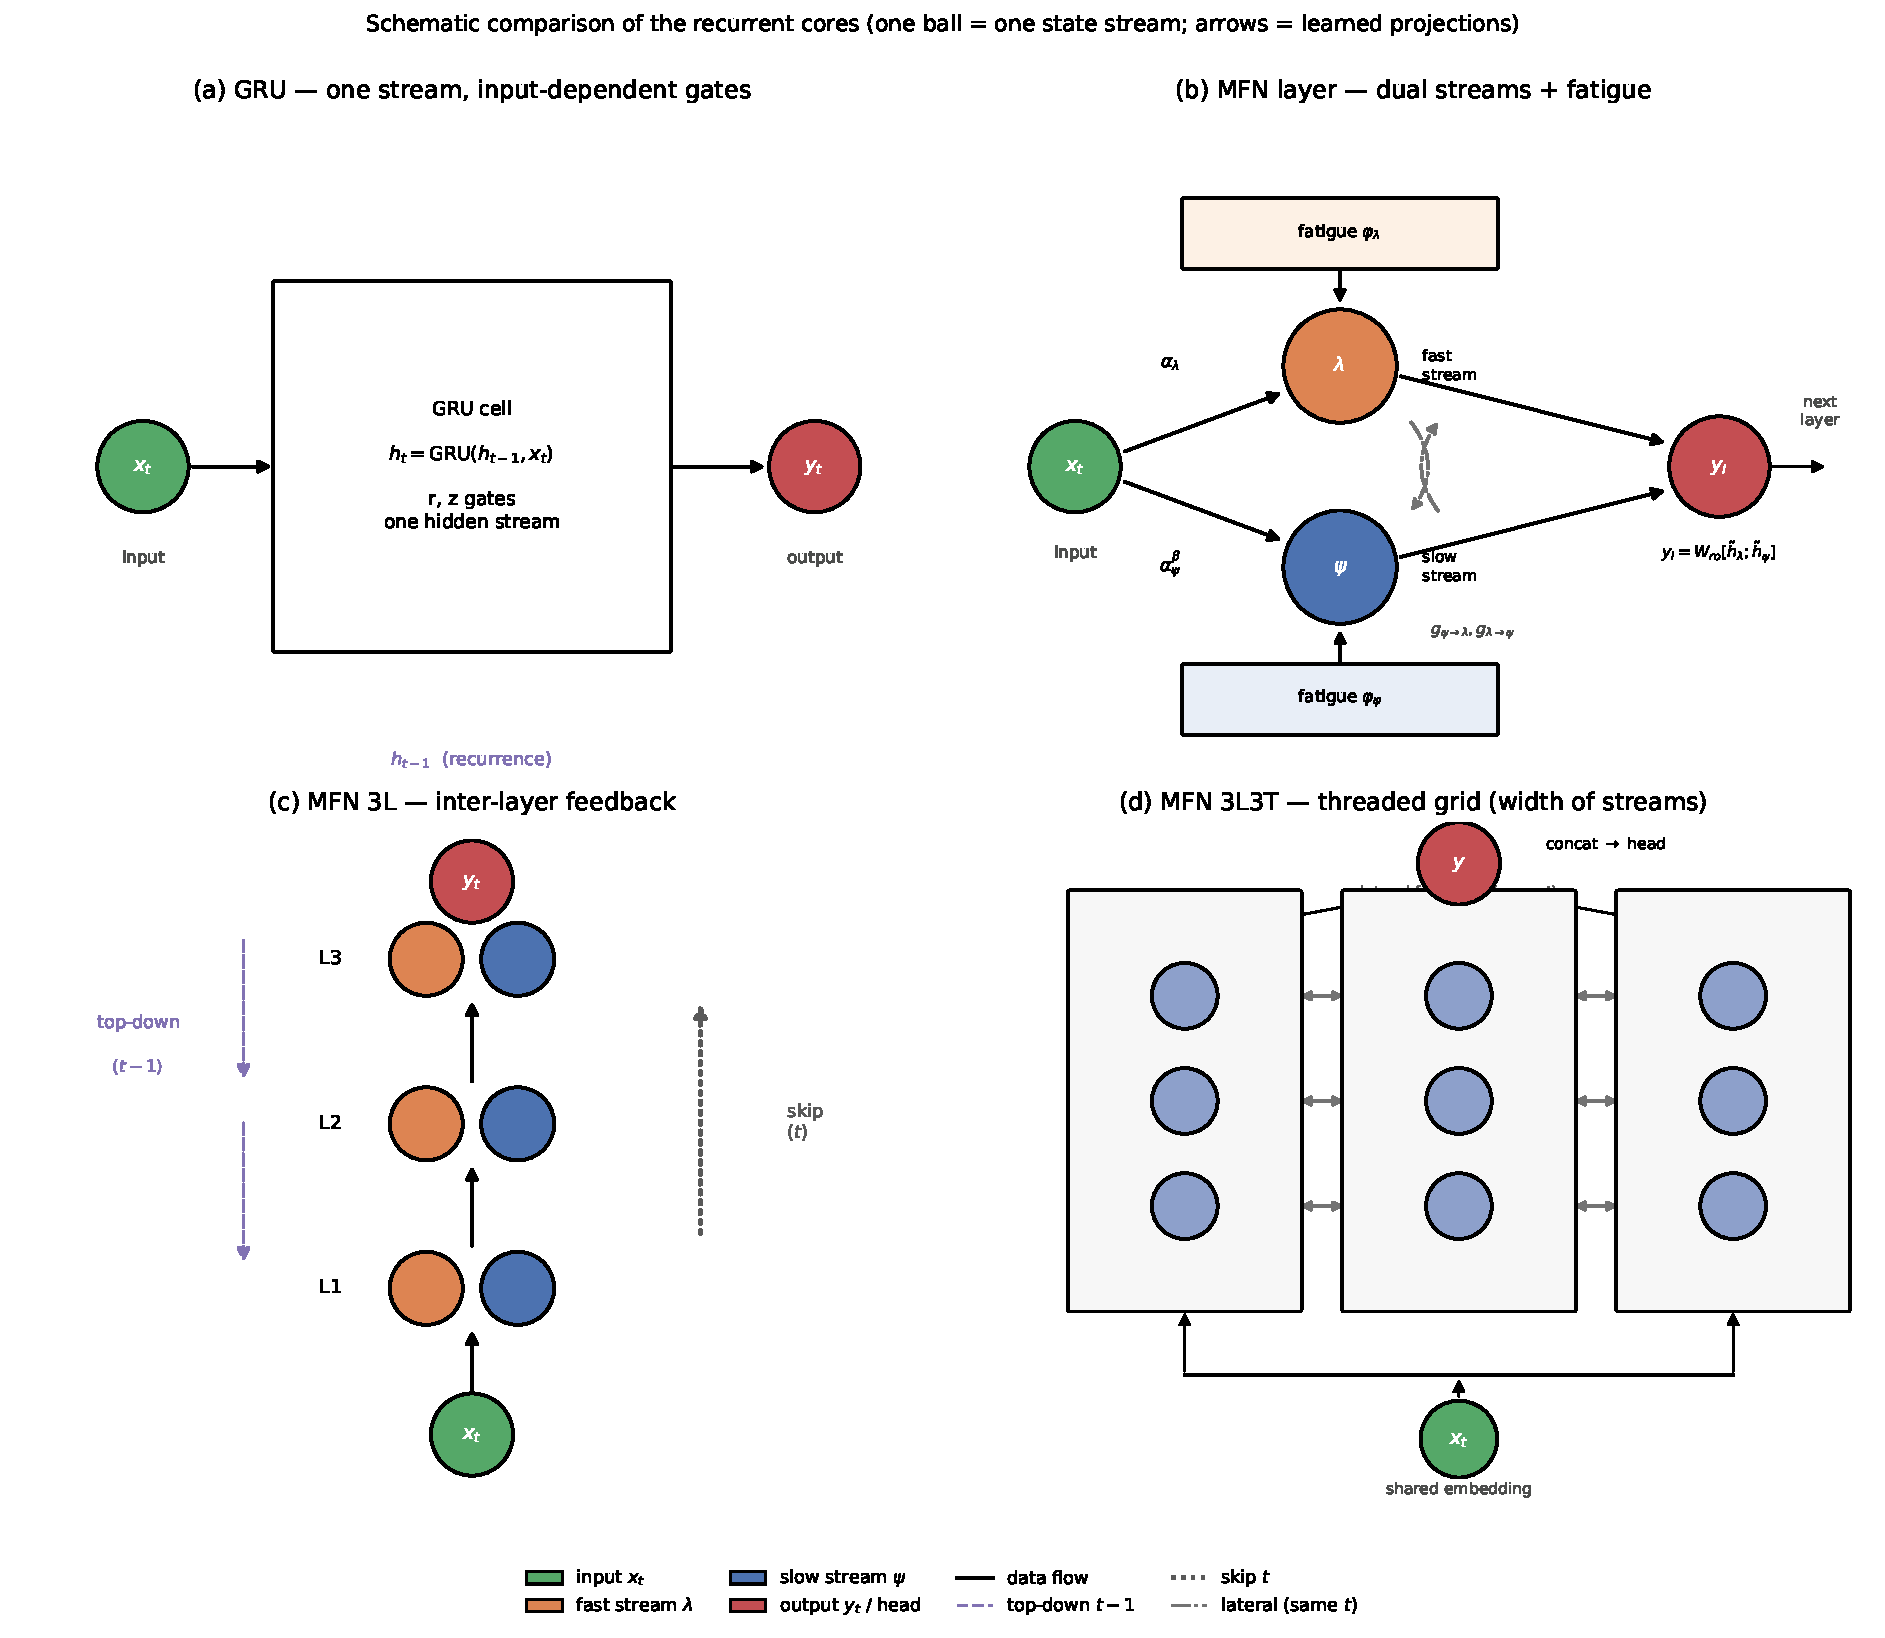
\includegraphics[width=0.88\textwidth]{arch_diagram.pdf}
\caption{\small Schematic comparison of the four recurrent cores discussed
in this paper: (a) GRU baseline; (b) MFN dual-stream layer (fast
$\lambda$-stream in orange, slow $\psi$-stream in blue, fatigue
accumulators, exponentiated decay $\alpha_\psi^{\beta}$, cross-stream
gates); (c) MFN 3L with top--down ($t-1$) and skip ($t$) feedback;
(d) MFN 3L3T threaded grid with lateral feedback at every stage and
concatenating readout.}
\label{fig:arch}
\end{figure}

\section{Mechanisms of the feedback paths}\label{sec:mech}
Figure~\ref{fig:mech} makes the two feedback mechanisms explicit.
\paragraph{Inter-layer (Fig.~\ref{fig:mech}a).} The stack is unrolled over
two time steps $t-1$ and $t$ for three layers $L1$ (shallow) to $L3$
(deep). Data flows bottom-up within each time step (feed-forward
$y_l \to u_{l+1}$, solid arrows). Two feedback channels recur:
\emph{top--down}: the deeper layer's readout $y_{l+1}$ at $t-1$ is projected
($\mathrm{td} = W_{td} y_{l+1}(t-1)$, dashed) and injected into layer $l$'s
mixture at step $t$, gated per neuron by $\sigma(u \odot \tilde h + v \odot
\mathrm{td} + b)$---a \emph{slow} channel (one step delayed), through which
deep representations steer shallow processing; \emph{skip}: the fresh
surface readout $y_0$ at $t$ (dotted) is injected into layers $l \ge 2$ in
the same step---a \emph{fast} channel that lets the surface guide deep
processing immediately. Both channels enter the $\lambda$ and $\psi$
mixtures with their own gate parameters (Eqs.~\eqref{eq:td}--\eqref{eq:mixpsi}).
\paragraph{Inter-thread (Fig.~\ref{fig:mech}b).} At each layer $l$, after
all $K$ threads computed their readouts $y_l^{(k)}$, every thread receives
gated lateral projections from the others (Eq.~\eqref{eq:lateral}) before
feeding layer $l+1$ (and the head). The exchange happens at the same time
step $t$, with a separate learned gate $(u^{(kj)}, v^{(kj)}, b^{(kj)})$ per
ordered pair, so a thread may listen more to one neighbor than another; the
per-neuron sigmoid gate makes the coupling selective rather than additive.

\begin{figure}[t]\centering
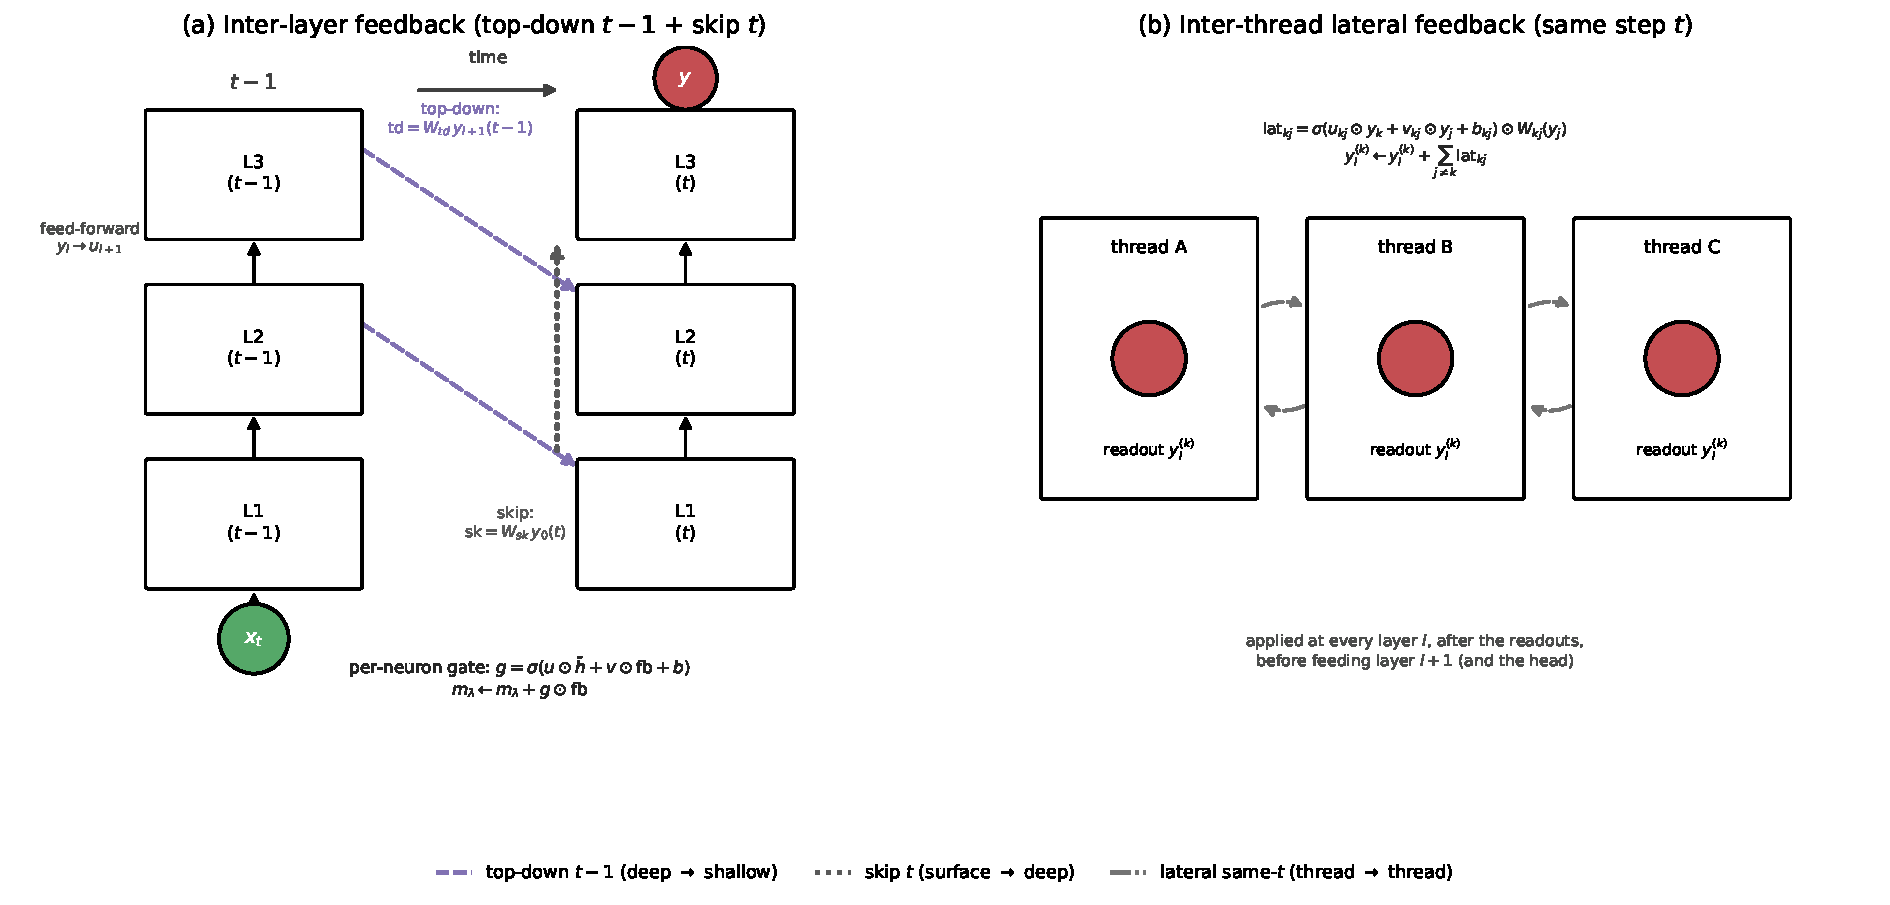
\includegraphics[width=0.94\textwidth]{feedback_mech.pdf}
\caption{\small Mechanisms of the feedback paths: (a) inter-layer feedback
as a time unrolled schematic ($t-1$ and $t$ columns; $L1$--$L3$ layers;
dashed purple = top--down from $y_{l+1}(t-1)$, dotted = skip from
$y_0(t)$, with the per-neuron gate formula); (b) inter-thread lateral
feedback at one layer: three threads exchange gated projections of their
readouts (Eq.~\eqref{eq:lateral}) before layer $l+1$.}
\label{fig:mech}
\end{figure}

\section{Training methodology}\label{sec:training}
\textbf{Objective.} Standard next-token cross-entropy over the corpus.
\textbf{Optimizer.} AdamW ($\beta_1=0.9$, $\beta_2=0.999$,
weight decay $0.1$), gradient norm clipped to $1.0$; per-epoch warm-up of 200
steps followed by a cosine decay; learning rates $10^{-3}$ (matched
protocol) or $5\times10^{-4}$ (exploration runs, explicitly marked).
\textbf{Robustness guards.} Beyond the clamp of \S\ref{sec:stability}, every
training step is guarded: (i) a shadow copy of the weights is refreshed after
each successful step; (ii) a step is declared \emph{bad} and rolled back if
the loss is non-finite, if $\ell > 4\,\mathrm{EMA}(\ell) + 4$ (outlier
batch), or if the gradient norm is non-finite; (iii) training aborts cleanly
after 50 consecutive bad steps. These guards make the failure mode
\emph{benign}: a pathological batch can no longer corrupt the model state,
it is skipped.
\textbf{Comparison validity rules.} A comparison between two runs is valid
only if: identical corpus, tokenizer, seed, and sequence layout; matched
epoch budgets; matched learning rates. Runs failing any of these (e.g., the
$5\times10^{-4}$ phase-5 family, or runs interrupted and resumed with fresh
optimizer state) are reported as observations but \emph{excluded} from
scaling fits.

\section{Experimental setup}\label{sec:setup}
\textbf{Data.} A fixed subset of TinyStories \citep{eldan2023tinystories}:
22.6\,M tokens (100k stories), BPE tokenizer of size 4096, train / val /
test splits fixed; every model in the paper sees the identical byte-stream,
in the identical order (no per-epoch shuffling), seed~0.
\textbf{Baselines.} GRU with layer norm (H=215, 1\,159\,710
parameters) and GPT-2-mini (4 layers $\times$ 120, 1\,250\,640 parameters),
both trained with the same protocol at $10^{-3}$ for 4 epochs (GPT-2-mini:
6).
\textbf{Models.} See Table~\ref{tab:models}. Parameter counts are measured
(sum of tensor elements after deduplication of tied weights), not
estimated.
\textbf{Hardware.} Single NVIDIA GTX 960M (Maxwell, 2\,GB), 4 CPU cores.
This constrains batch sizes (activations of the unrolled recurrent graph
dominate the memory budget) and prevents fp16 acceleration; all numbers are
fp32.

\begin{table}[t]\centering\small
\caption{Model family. $\dagger$: intermittent training history (bugged
epochs) --- reported, not used in scaling fits.}\label{tab:models}
\begin{tabular}{lcccc}
\toprule
Model & Widths & Threads & Parameters & Status \\
\midrule
MFN 1L & $[144]$ & 1 & 1\,153\,440 & trained, $10^{-3}$, 4 ep \\
GRU & $[215]$ & -- & 1\,159\,710 & trained, $10^{-3}$, 4 ep \\
GPT-2 mini & $4\times120$ & -- & 1\,250\,640 & trained, $10^{-3}$, 6 ep \\
MFN 2L & $[192,96]$ & 1 & 2\,122\,368 & trained $5\!\times\!10^{-4}$, 4 ep$^\dagger$ \\
MFN 3L & $[192,128,96]$ & 1 & 2\,612\,384 & trained $5\!\times\!10^{-4}$, 3 ep \\
MFN 3L$_{1e-3}$ & $[192,128,96]$ & 1 & 2\,612\,384 & trained $10^{-3}$, 4 ep --- val 2.4135, test ppl 11.39 \\
MFN 2ZF & $2\times[160,112,80]/[96,64,48]$ & 2 & 1\,814\,000 & trained $10^{-3}$, 2 ep --- val 2.5352, test ppl 12.85 \\
MFN 3L3T & $[192,128,96]$ & 3 & 6\,753\,888 & scheduled \\
\bottomrule
\end{tabular}
\end{table}

\section{Results}\label{sec:results}
\subsection{Equal-size comparison (phase 4 protocol, $10^{-3}$, matched)}
Table~\ref{tab:baselines} shows test perplexity after the matched budget.
At equal parameter count and identical protocol, MFN 1L beats the GRU by
$0.034$ nat and GPT-2-mini by $0.96$ nat on test loss.

\begin{table}[t]\centering\small
\caption{Phase-4 baselines: validation loss per epoch and test perplexity.
All at $10^{-3}$, identical data order, seed 0.}\label{tab:baselines}
\begin{tabular}{lccccr}
\toprule
Model & ep1 & ep2 & ep3 & ep4 & Test ppl \\
\midrule
MFN 1L (1\,153\,440) & 2.6988 & 2.5269 & 2.4477 & 2.4013 & 11.20 \\
GRU (1\,159\,710) & 2.6583 & 2.5280 & 2.4708 & 2.4351 & 11.58 \\
GPT-2 mini (1\,250\,640) & 3.6818 & 3.4976 & 3.4334 & 3.3968 & 29.41 (ep6) \\
\bottomrule
\end{tabular}
\end{table}

\subsection{Depth family at equal stage}\label{sec:depth}
Within the $5\times10^{-4}$ family (valid only between the two deep runs),
MFN 3L beats MFN 2L at every shared epoch (Table~\ref{tab:depth}): depth
continues to pay at matched budgets. Both runs remain ineligible for scaling
fits (learning-rate mismatch and interrupted history).

\begin{table}[t]\centering\small
\caption{Validation loss by epoch, phase-5 family ($5\times10^{-4}$). The
3L run uses 3 epochs; a 4th epoch was added later and is pending.}
\label{tab:depth}
\begin{tabular}{lcccc}
\toprule
Model & ep1 & ep2 & ep3 & Test ppl \\
\midrule
MFN 2L (2\,122\,368) & 3.0371 & 2.8161 & 2.6903 & 13.75 \\
MFN 3L (2\,612\,384) & 3.0541 & \textbf{2.7945} & \textbf{2.6582} & 14.53 \\
\bottomrule
\end{tabular}
\end{table}

\subsection{The FAST zone model (2ZF)}\label{sec:2zf}
\paragraph{Motivation.} The dense dual-stream cell spends $45\%$ of its
FLOPs in two per-stream \texttt{GRUCell}s whose update gate $z$ duplicates
the input-conditioned decay $\alpha$ already computed by the cell's own
MLPs (the architecture's original paper already described
$h \leftarrow \alpha \odot h + (1-\alpha)\odot\tanh(\text{mix})$ as the
recurrence, Mamba-$\Delta$-style). \textbf{FAST cell:} we replace both GRUs
by $\alpha$-recurrence per stream, keep the $\tanh$ candidate, let the
fatigue accumulator $\varphi$ play the \emph{reset} role
($\tilde h = h \odot (1-\varphi)$), and fuse pairing operations into single
kernels (gates $2H{\to}2H$, cross-stream, within-stream feedback); the per-
layer cost drops from $\sim$22$H^2$ to $\sim$9$H^2$.
\paragraph{Learned temporal zones.} The two asymmetric zones
($A$: widths $[160,112,80]$, $\beta{=}0.2$, computed every step; $B$:
$[96,64,48]$, $\beta{=}0.6$, updated on alternate steps --- state-hold with
bounded error $\leq 2(1-\alpha_B)$, amortized by the slow stream's
integrative dynamics) instantiate a \emph{learned} clockwork hierarchy per
zone rather than per fixed neuron groups.
\paragraph{Measurements (22.6\,M tokens, $10^{-3}$, B64).}
Throughput 2\,202 tok/s --- 2.6$\times$ the dense zone model (849 tok/s),
matching the theory's prediction (1\,826--2\,739). At equal epochs the
1.81\,M-parameter 2ZF \emph{beats} the 2.61\,M 3L:
\begin{center}\small
\begin{tabular}{lcccc}
\toprule
Model & params & ep1 val & ep2 val & final \\ \midrule
MFN 3L & 2\,612\,384 & 2.8317 & 2.6017 & val 2.4135 (4 ep), ppl 11.39 \\
\textbf{MFN 2ZF} & \textbf{1\,814\,000} & \textbf{2.7765} & \textbf{2.5352} & test ppl 12.85 (2 ep) \\
\bottomrule
\end{tabular}
\end{center}
$\Rightarrow$ the GRU cells did not carry capacity (falsifiable prediction
\#2 of the theory, \texttt{phase5/THEORY\_2Z\_FAST.md}, confirmed); the
$\alpha$-recurrence + fatigue is both cheaper and per-epoch better at equal
protocol. The 2ZF is currently the base for the instruction-following
(UltraChat) SFT and for the 10-stage asymmetric depth test (Z10).

\subsection{Data exponent $\alpha_D$}\label{sec:ad}
For each model, we fit $\log L = a + \alpha_D \log D$ over the validation
losses of the first four epochs ($D$ = tokens seen).
\begin{figure}[t]\centering
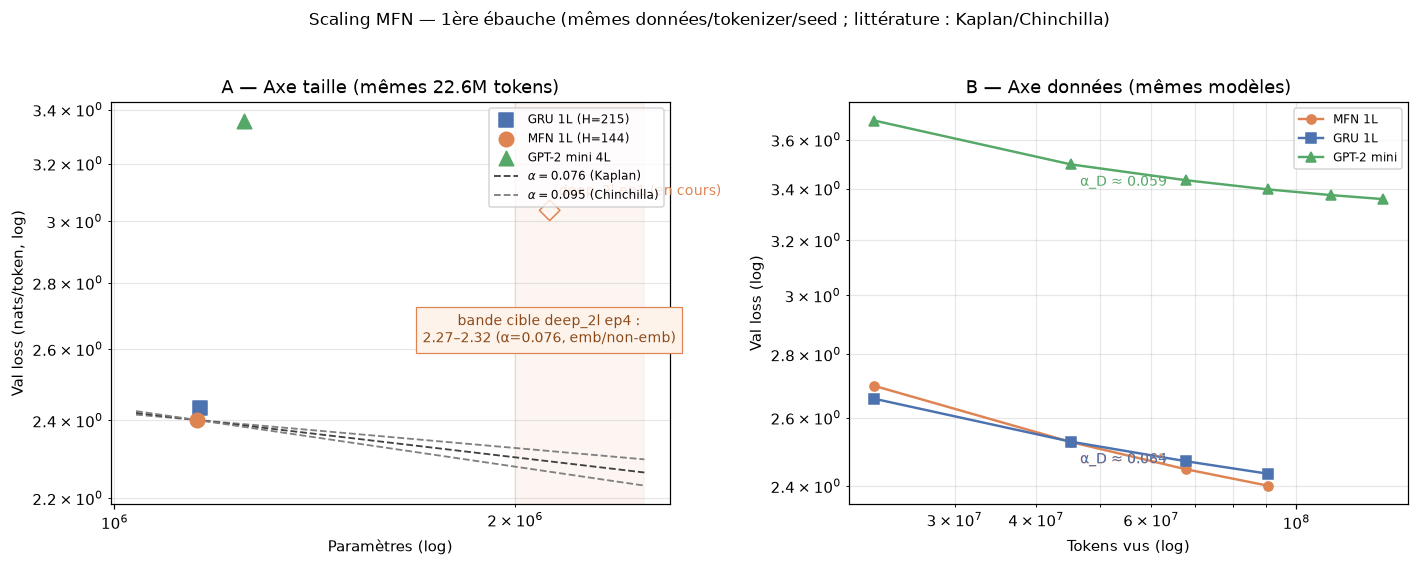
\includegraphics[width=0.98\textwidth]{scaling_curve.png}
\caption{\small Scaling evidence: (A) validation loss vs.\ parameters with the
reference slopes $\alpha\in\{0.057,0.076,0.095\}$ anchored at MFN 1L; (B)
validation loss vs.\ tokens seen with fitted local exponents $\alpha_D$
(MFN $\approx 0.085$, GRU $\approx 0.064$, GPT-2-mini $\approx 0.051$). The
shaded wedge marks the falsifiable band for the running 3L$_{1e-3}$ run
(\texttt{phase5/scaling\_curve.png}).}
\label{fig:scaling}
\end{figure}
\begin{table}[t]\centering\small
\caption{Local data exponents (fit over 4 epochs).}
\label{tab:alphad}
\begin{tabular}{lc}
\toprule
Model & $\alpha_D$ \\
\midrule
\textbf{MFN 1L} & \textbf{0.085} \\
GRU & 0.064 \\
GPT-2 mini & 0.051 \\
\emph{transformers (published)} & \emph{$\approx 0.095$} \\
\bottomrule
\end{tabular}
\end{table}
MFN extracts 33\% more loss reduction per token than the GRU and 65\% more
than GPT-2-mini on this corpus. The absolute value sits close to the
published transformer range \citep{kaplan2020scaling}, and the comparison is
protocol-matched---the same data, same tokenizer, same seed, same total
token budget per epoch.

\subsection{Robustness case study}\label{sec:robust}
Three runs collapsed at different learning rates ($10^{-3}$ and
$5\times10^{-4}$) in regions where the instantaneous loss hovered near
$3.0$--$3.05$ nat. Autopsy with
\texttt{torch.autograd.set\_detect\_anomaly} isolated the exact backward
operation: $\mathrm{SigmoidBackward0}$ returning NaN in
\eqref{eq:decays}. The forward pass was always finite---the signature of a
\emph{derivative cliff}, not a corrupted weight or a data artifact (the
batch statistics of the affected data zone were checked and are normal).
After the clamp of \S\ref{sec:stability}, the subsequent 4 epochs
accumulated \textbf{zero} rollbacks while improving validation loss
monotonically. The methodological lesson: repeated collapse at identical
\emph{data positions} across runs is evidence of a deterministic cause
(data order is fixed; the state is not) --- gradient-anomaly tracing is the
decisive tool.

\subsection{Preregistered falsifiable prediction --- result}\label{sec:prereg}
The parameter exponent $\alpha_N$ was estimated from the matched pair
$P_0$ (MFN 1L, 1\,153\,440) and $P_4$ (MFN 3L, 2\,612\,384), both at
$10^{-3}$ for 4 epochs on the identical 22.6\,M-token stream. With
$L(N) = A N^{-\alpha_N}$, the bar $\alpha_N \ge 0.076$ (Kaplan et al.)
requires $L_{P_4} \le 2.4013 \times (2.612/1.153)^{-0.076} \approx 2.26$ on
total parameters, or $\le 2.20$ on non-embedding parameters (ratio
$3.24\times$). The prediction was written to \texttt{phase5/scaling.md}
before the run; an earlier draft printed $\approx 2.30$, an arithmetic error
($+0.044$ nat).

\textbf{Outcome: the bar is falsified.} Final validation loss of the 3L run:
$\mathbf{2.4135}$ (ppl 11.17; test ppl 11.39, vs.\ MFN~1L 11.20 and GRU
11.58). The measured local exponent is $\alpha_N = -0.006$ (total params) /
$-0.004$ (non-embedding)---flat at this scale. Three observations frame this
result. \emph{(i) Per-epoch gains decay geometrically}: $-0.230$, $-0.116$,
$-0.072$ from epochs 1--4 (ratio $\approx 0.5$--$0.62$); extrapolating the
geometric tail puts the corpus asymptote near $2.30$, still above the bar ---
more epochs at fixed data could not have reached it. \emph{(ii) Data
starvation, not architecture}: at 22.6\,M tokens the 3L sees
$8.65$ tokens/parameter versus $19.6$ for the 1L ($2.3\times$ below the
Chinchilla-optimal ratio); added capacity cannot express itself in this
regime, and the depth family indeed converges toward the 1L's loss rather
than past it. \emph{(iii) The learning-rate effect holds independently}: the
$10^{-3}$ run beats its $5\times10^{-4}$ twin at every matched epoch
($-0.22$, $-0.19$, $-0.17$, $-0.14$), so the comparison is not a
convergence artifact. The preregistered prediction did its job: it was
falsifiable, and it was falsified. The measurement programme now moves to
the data axis (\S\ref{sec:discussion}): a $\sim$2--3$\times$ larger unique
corpus at $\approx$1 epoch is the cleanest test of whether MFN's
$\alpha_N$ emerges once tokens/parameter approaches the Chinchilla ratio.

\section{Discussion and scaling programme}\label{sec:discussion}
\paragraph{Axis D (data).} $\alpha_D \approx 0.085$ (measured, local).
Target: confirm across sizes; the corpus is $\approx 10.7$ tokens/parameter
at 2.1M parameters, i.e., below the Chinchilla-optimal $\approx 20$
\citep{hoffmann2022chinchilla}; more unique data at matched token budget is
the highest-ROI axis.
\paragraph{Axis N (parameters).} The matched pair $P_0$/$P_4$ is complete:
the preregistered bar is \emph{falsified} at this data budget
($\alpha_N \approx -0.01$; \S\ref{sec:prereg}). We read this as a
data-limited regime (8.65 tokens/parameter, $2.3\times$ below Chinchilla),
so the next $\alpha_N$ measurement requires a larger unique corpus first.
Two-point fits are fragile; the reconciliation
literature \citep{pearce2024reconciling,porian2024data} warns of
small-scale curvature, so any $\alpha_N$ we report is a \emph{local}
exponent.
\paragraph{Axis depth vs. width of streams.} Depth pays at matched stages
(\S\ref{sec:depth}); the multi-thread grid 3L3T tests whether the
\emph{width of streams} axis ($K$ parallel coupled stacks, \S\ref{sec:threads})
keeps paying where sequential depth might saturate---the classical RNN depth
barrier. An ablation of the lateral coupling isolates its contribution.
\paragraph{Axis context.} Per-token cost is $O(H)$ in sequence length for
recurrence, versus $O(n^2)$ (and KV growth) for attention. Kaplan et al.\
report that LSTMs match transformers early in context and degrade later
\citep{kaplan2020scaling}; MFN's dual-scale design is the direct attempt to
avoid exactly that degradation, and a long-context measurement
(256/512-length evaluations at fixed budget) is the cleanest arena for the
architecture's claim.
\paragraph{Caveats.} (i) exponents are local (below $10^8$ parameters);
(ii) the gating overhead raises per-token FLOPs, so the compute-adjusted
curve may be less flattering than the parameter-adjusted one; (iii)
transformers' exponents reflect eight years of training-recipe engineering,
while MFN's recipes are younger; (iv) all baselines here are small-scale and
in-domain---claims are about \emph{relative} behavior on this corpus.

\section{Conclusion}\label{sec:conclusion}
We described the Memory--Fatigue Network---dual-scale recurrent layers with
learned fatigue, per-neuron gated top--down / skip / lateral feedback---and
a controlled small-scale measurement protocol. Current evidence: MFN
outperforms GRU and GPT-2-mini baselines at equal size and budget; its local
data exponent is steeper than both; a single numerical cliff, root cause of
three collapses, is identified and eliminated. The preregistered parameter
exponent test completed and was falsified: at 8.65 tokens/parameter, depth
converges to the single-layer loss ($\alpha_N \approx -0.01$) --- a data
starvation signature rather than an architectural verdict, which redirects
the programme to the data axis. If MFN's exponents match or exceed the
published ones once tokens/parameter approaches the Chinchilla ratio, the
``scaling barrier" is not a law of nature but a property of inductive
biases---and fatigue-driven multi-scale recurrence is a candidate for
shifting it.

\bibliographystyle{abbrv}
\begin{thebibliography}{99}
\bibitem[Ba et al.(2016)]{ba2016highway} R.~K. Ba, R.~Hjelm, K.~Cho.
Highway networks. Deep Learning Workshop, ICML 2016.
\bibitem[Cho et al.(2014)]{cho2014gru} K.~Cho, B.~van~Merri\'enboer,
C.~Gulcehre, D.~Bahdanau, F.~Bougares, H.~Schwenk, Y.~Bengio. Learning
phrase representations using RNN encoder--decoder... EMNLP 2014.
\bibitem[Eldan and Li(2023)]{eldan2023tinystories} R.~Eldan, Y.~Li.
TinyStories: how small can language models be... arXiv:2305.07759, 2023.
\bibitem[Gu and Dao(2023)]{gu2023mamba} A.~Gu, T.~Dao. Mamba:
linear-time sequence modeling with selective state spaces. arXiv:2312.00752,
2023.
\bibitem[Hochreiter and Schmidhuber(1997)]{hochreiter1997lstm} S.~Hochreiter,
J.~Schmidhuber. Long short-term memory. Neural Computation 9(8), 1997.
\bibitem[Hoffmann et al.(2022)]{hoffmann2022chinchilla} J.~Hoffmann et al.
Training compute-optimal large language models. NeurIPS 2022.
\bibitem[Horn(1970)]{horn1970behavior} G.~Horn. Changes in neuronal
activity and behavior. Experimental Biology, 1970.
\bibitem[Kaplan et al.(2020)]{kaplan2020scaling} J.~Kaplan et al. Scaling
laws for neural language models. arXiv:2001.08361, 2020.
\bibitem[Koutn\'ik et al.(2014)]{koutnik2014clockwork} J.~Koutn\'ik,
K.~Greff, F.~Gomez, J.~Schmidhuber. A clockwork RNN. ICML 2014.
\bibitem[Mikolov et al.(2015)]{mikolov2014learning} T.~Mikolov,
A.~Joulin, S.~Chopra, M.~Courville, Y.~Bengio. Learning longer memory in
recurrent neural networks. ICLR 2015.
\bibitem[Pearce and Song(2024)]{pearce2024reconciling} T.~Pearce, J.~Song.
Reconciling Kaplan and Chinchilla scaling laws. arXiv:2406.12907, 2024.
\bibitem[Peng et al.(2023)]{peng2023rwkv} B.~Peng et al. RWKV: reinventing
RNNs for the transformer era. arXiv:2305.13048, 2023.
\bibitem[Porian et al.(2024)]{porian2024data} T.~Porian, M.~Wortsman,
J.~Li. Data quality scaling laws. arXiv:2410.19382, 2024.
\bibitem[Radford et al.(2019)]{radford2019language} A.~Radford et al.
Language models are unsupervised multitask learners. OpenAI Tech. Rep., 2019.
\bibitem[Shazeer et al.(2017)]{shazeer2017outrageously} N.~Shazeer et al.
Outrageously large neural networks: the sparsely-gated mixture-of-experts
layer. ICLR 2017.
\bibitem[Stopfer(1997)]{stopfer1997impaired} M.~Stopfer, Y.~Bhagavan,
B.~Smith, G.~Laurent. Impaired odour discrimination on desynchronization of
odour-encoding neural assemblies. Nature 390, 1997.
\bibitem[Vaswani et al.(2017)]{vaswani2017attention} A.~Vaswani et al.
Attention is all you need. NeurIPS 2017.
\end{thebibliography}
\end{document}